\documentclass{article}
\usepackage[ttscale=0.825]{libertine}
\usepackage[libertine]{newtxmath}
\usepackage{amsmath,amstext,amssymb}
\usepackage{graphicx}
\usepackage{sectsty}
\usepackage{siunitx}
\usepackage{parskip}
\usepackage{booktabs}
\usepackage{hyperref}
\hypersetup{colorlinks=true,urlcolor=blue}

\newcommand{\oderiv}[2]{\ensuremath{\frac{\text{d}#1}{\text{d}#2}}}

\begin{document}
\allsectionsfont{\normalfont\sffamily\bfseries}
\begin{center}
    \large{CVEN 306 Laboratory Exercise}

    \Large{\textsf{\textbf{Thermal Conduction in a Composite}}}

    \large{\textsf{Task 4 Solution}}
\end{center}

\vspace{0.25truein}
\subsection*{Task 4}
Design a three-layer composite wall with the \textit{minimum possible} effective heat transfer coefficient
subject to the following engineering constraints:
\begin{itemize}
    \item You must choose materials from among the three given in Table~1.
    \item $h_L = h_R = \SI{5}{\watt\per\meter\squared\per\kelvin}$.
    \item The wall must be \SI{1}{\meter} thick.
    \item The overall density of the wall must be between
        \SI{2.0}{\gram\per\centi\meter\cubed} and
        \SI{4.0}{\gram\per\centi\meter\cubed}.
\end{itemize}

\subsubsection*{Step 1: Write objective function}
The ordering of the materials does not matter, so we will just assume that layer 1
is PP, layer 2 is stainless steel, and layer 3 is aluminum.
The objective function in this case is Eq.~(6):
\begin{align}
    R = \frac{1}{U_{\text{e}}} &= \frac{1}{h_L} + \frac{L_1}{k_1} + \frac{L_2}{k_2}
    + \frac{L_3}{k_3} + \frac{1}{h_R} \nonumber \\
    &= \frac{1}{5} + \frac{L_1}{0.15} + \frac{L_2}{20} + \frac{1 - L_1 - L_2}{220} + \frac{1}{5}
    \nonumber \\
    &= 0.4 + 6.667 L_1 + 0.05 L_2 + 0.00455 - 0.00455 L_1 - 0.00455 L_2 \nonumber \\
    R &= 0.4046 + 6.6622 L_1 + 0.0455 L_2
    \label{eq:objectivefn}
\end{align}

\subsubsection*{Step 2: Write the constraints as linear inequalities}

\textbf{Constraint 1}:  The density must be at least \SI{2.0}{\gram\per\centi\meter\cubed}, which
can be written as
\begin{align*}
    0.9 L_1 + 7.8 L_2 + 2.7 \left( 1 - L_1 - L_2 \right) &\ge 2 \\
    2.7 - 1.8 L_1 + 5.1 L_2 &\ge 2 \\
    L_2 &\ge 0.3529 L_1 - 0.1373
\end{align*}

\textbf{Constraint 2}:  The density must be no greater than \SI{4.0}{\gram\per\centi\meter\cubed}, which
can be written as
\begin{align*}
    0.9 L_1 + 7.8 L_2 + 2.7 \left( 1 - L_1 - L_2 \right) &\le 4 \\
    2.7 - 1.8 L_1 + 5.1 L_2 &\le 4 \\
    L_2 &\le 0.3529 L_1 + 0.2549
\end{align*}

\textbf{Constraint 3}: The sum of the first two layer thicknesses cannot exceed the wall thickness,
which means
\[
    L_2 \le 1 - L_1
\]

\textbf{Constraints 4 and 5}: None of the wall thicknesses can be negative:
\begin{align*}
    L_1 &\ge 0 \\
    L_2 &\ge 0
\end{align*}

To summarize, here are the constraints:
\begin{align}
    L_2 &\ge 0.3529 L_1 - 0.1373 \\
    L_2 &\le 0.3529 L_1 + 0.2549 \\ 
    L_2 &\le 1 - L_1 \\
    L_1 &\ge 0 \\
    L_2 &\ge 0
\end{align}

\subsubsection*{Step 3: Plot all the inequalities on the same graph}

\begin{center}
    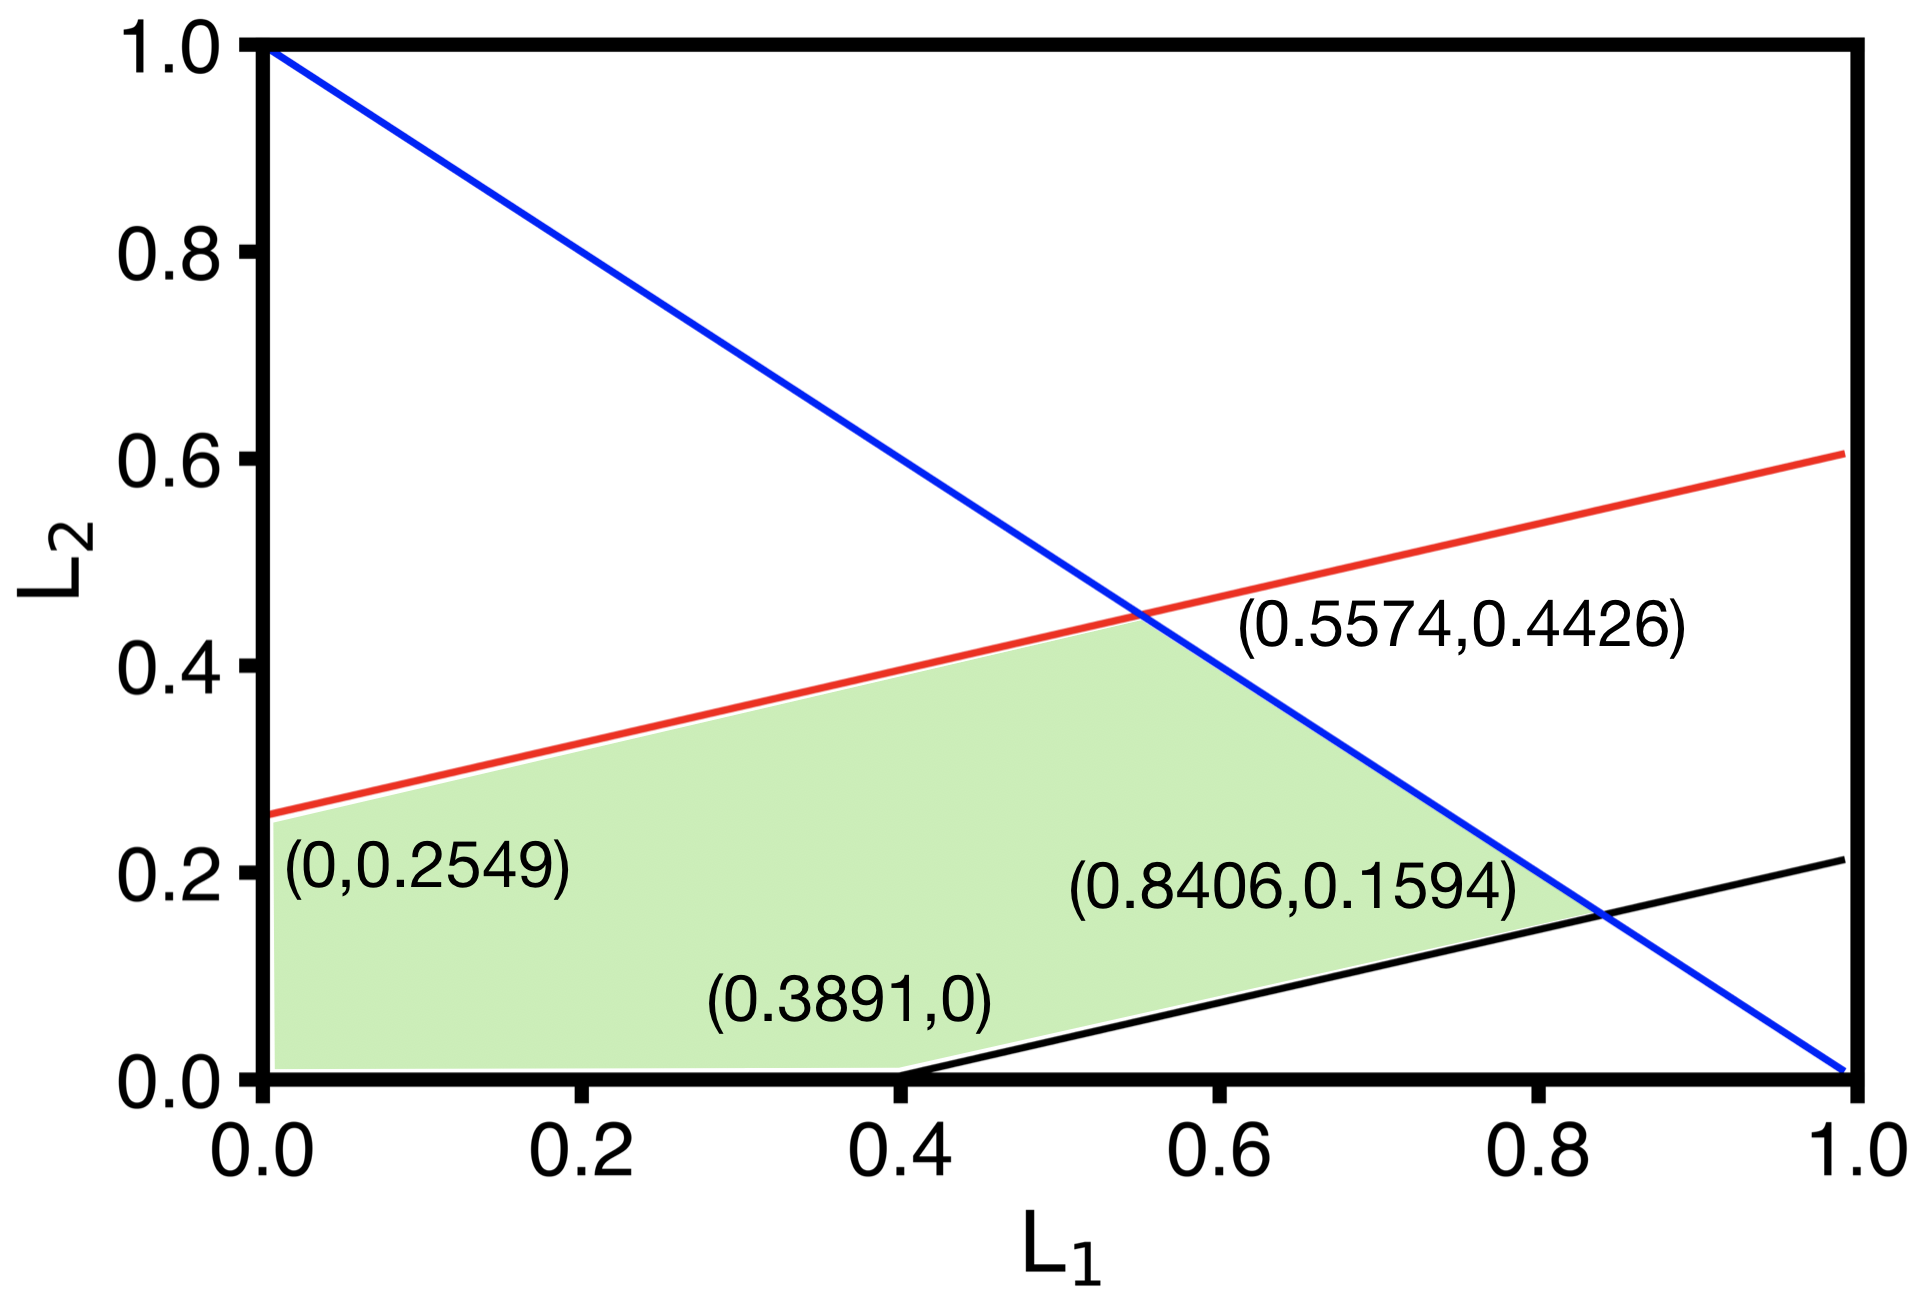
\includegraphics[scale=0.4]{Task4Plot.png}
\end{center}

\subsubsection*{Step 3: Test the vertices}

\begin{center}
\begin{tabular}{lll} \toprule
Vertex $(L_1,L_2)$ & Value of $R = 1/U$ & Diagnosis \\ \midrule
$(0,0)$ & $0.4046$ & Minimum \\
$(0,0.2549)$ & $0.4162$ & \\
$(0.5574,0.4426))$ & $4.1382$ & \\
$(0.8406,0.1594)$ & $6.0121$ & Maximum \\
$(0.3891,0)$ & $2.9969$ & \\ \bottomrule
\end{tabular}
\end{center}

The maximum of the objective function is $R=6.0121$ and it occurs when
$L_1 = 0.8406$, $L_2 = 0.1594$, $L_3 = 0$.  In this configuration,
the miminum value of $U_{\text{e}} = 1/R = \SI{0.1663}{\watt\per\meter\squared\per\kelvin}$,
and the density is \SI{2}{\gram\per\centi\meter\squared}.

\end{document}
